\chapter{Gráficas de análisis de integrador fraccionario con CFE}

%-------------------------------------------------------------------------------
%                            Graficas sin normalizar                           %
%-------------------------------------------------------------------------------
\begin{figure}[hbtp]
	\caption{Diagramas de magnitud de aproximaciones de integrador fraccionario general.}
	\centering
	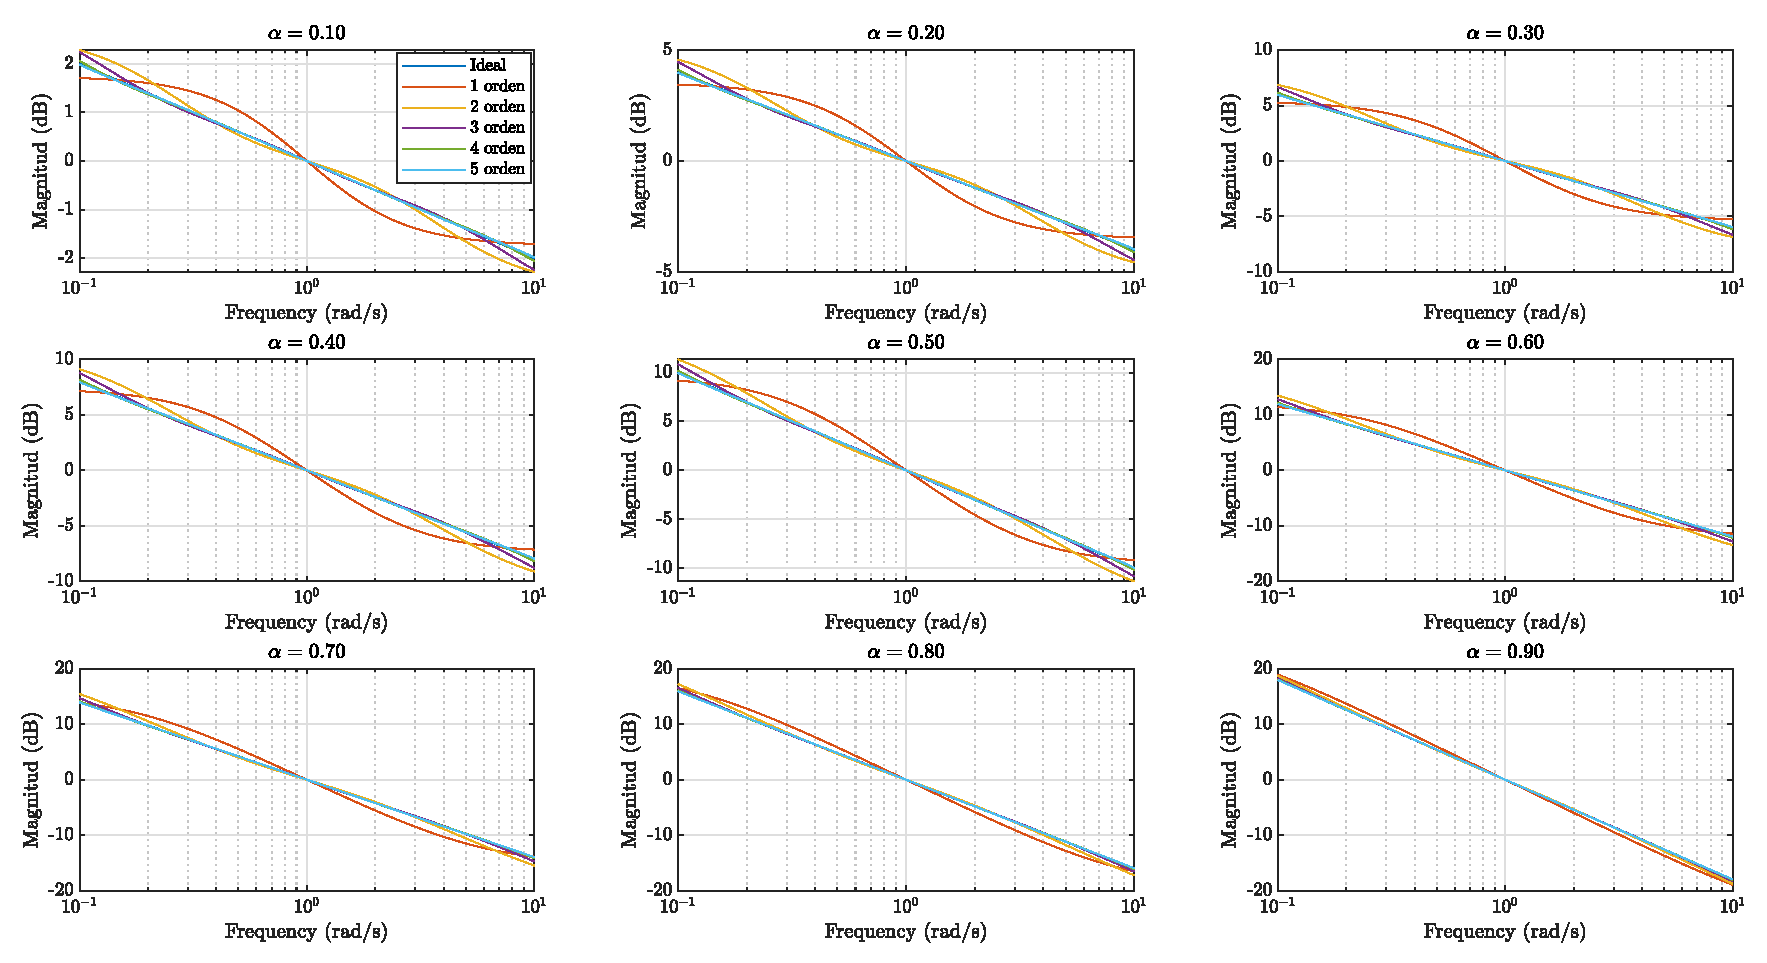
\includegraphics[width=0.93\textheight,angle=90]{F2_bode_magnitud_c.eps}
\end{figure}

\begin{figure}[hbtp]
	\caption{Diagramas de fase de aproximaciones de integrador fraccionario general.}
	\centering
	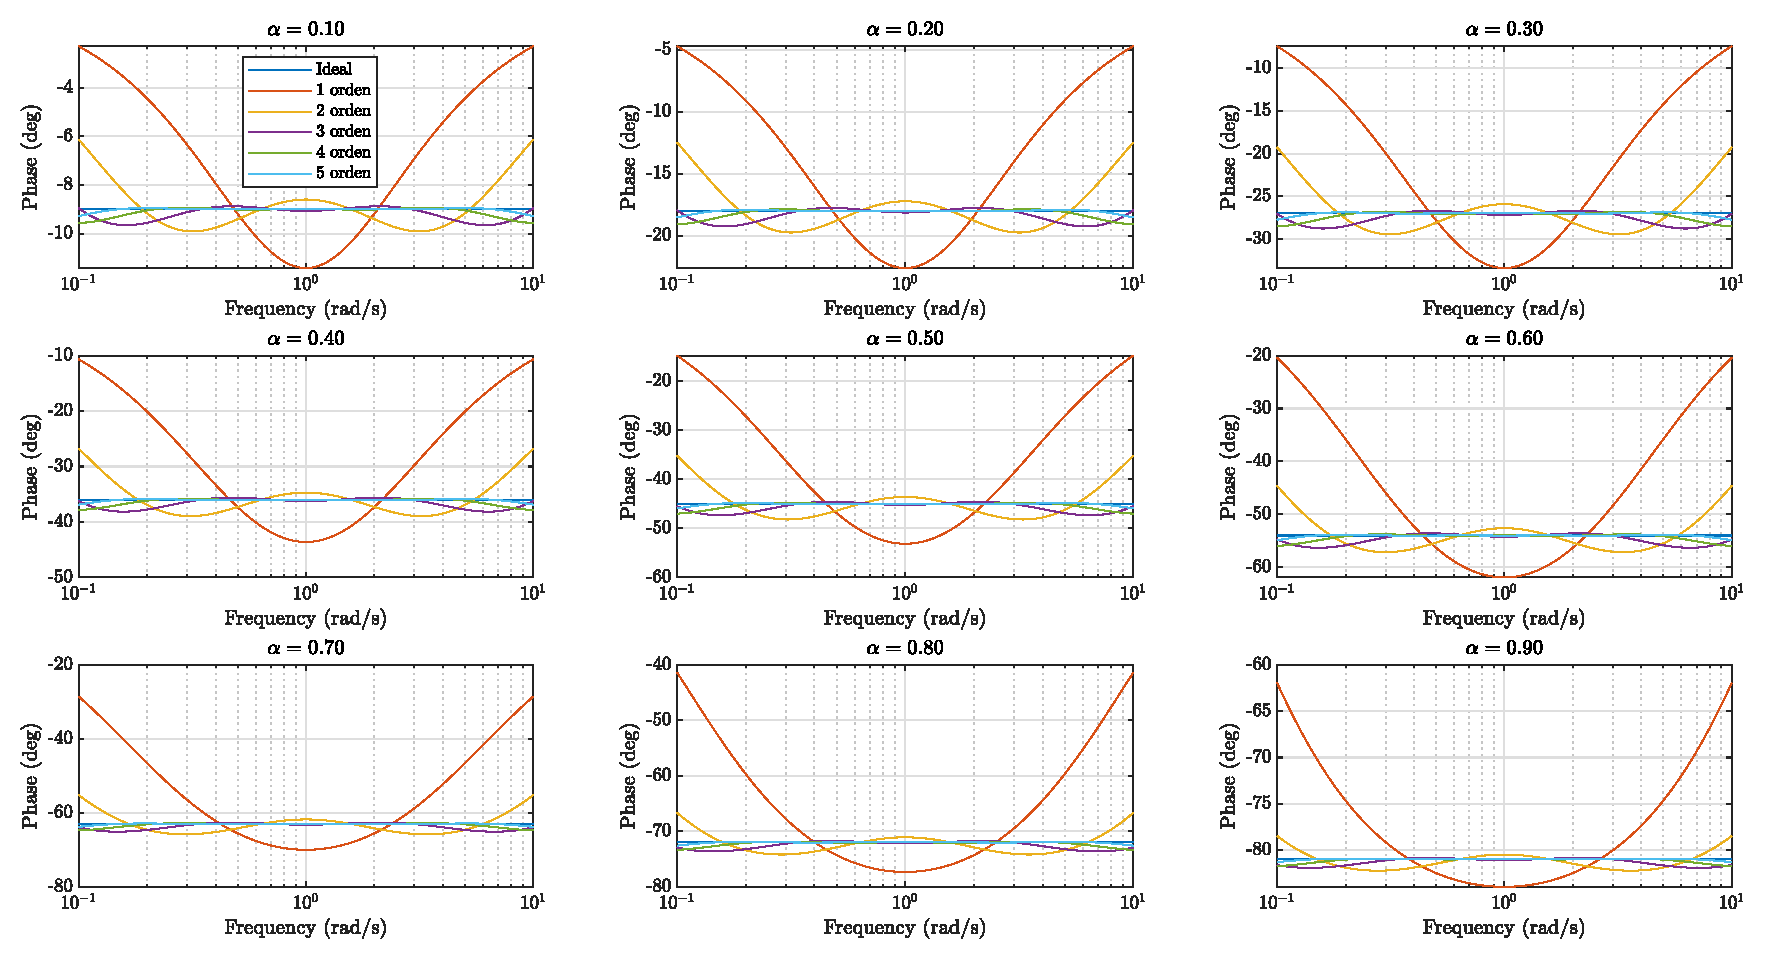
\includegraphics[width=0.93\textheight,angle=90]{F3_bode_fase_c.eps}
\end{figure}

\begin{figure}[hbtp]
	\caption{Diagramas de error de magnitud de aproximaciones de integrador fraccionario general.}
	\centering
	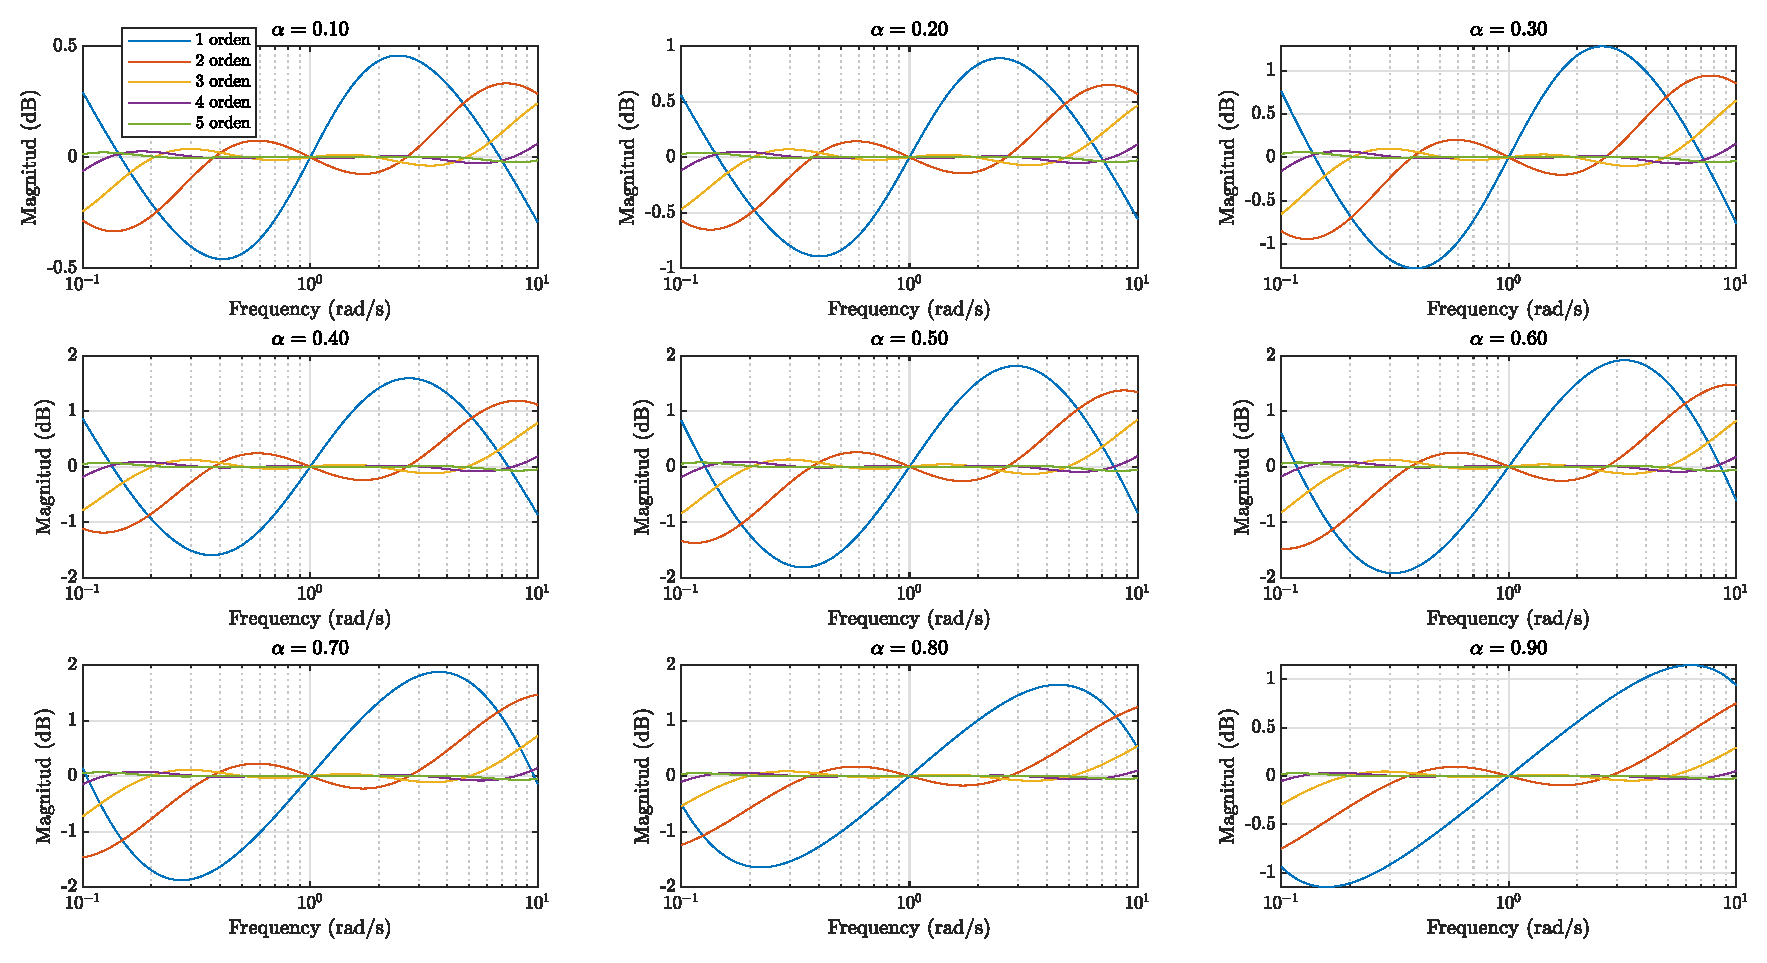
\includegraphics[width=0.93\textheight,angle=90]{F4_bode_error_mag_c.eps}
\end{figure}

\begin{figure}[hbtp]
	\caption{Diagramas de error de fase de aproximaciones de integrador fraccionario general.}
	\centering
	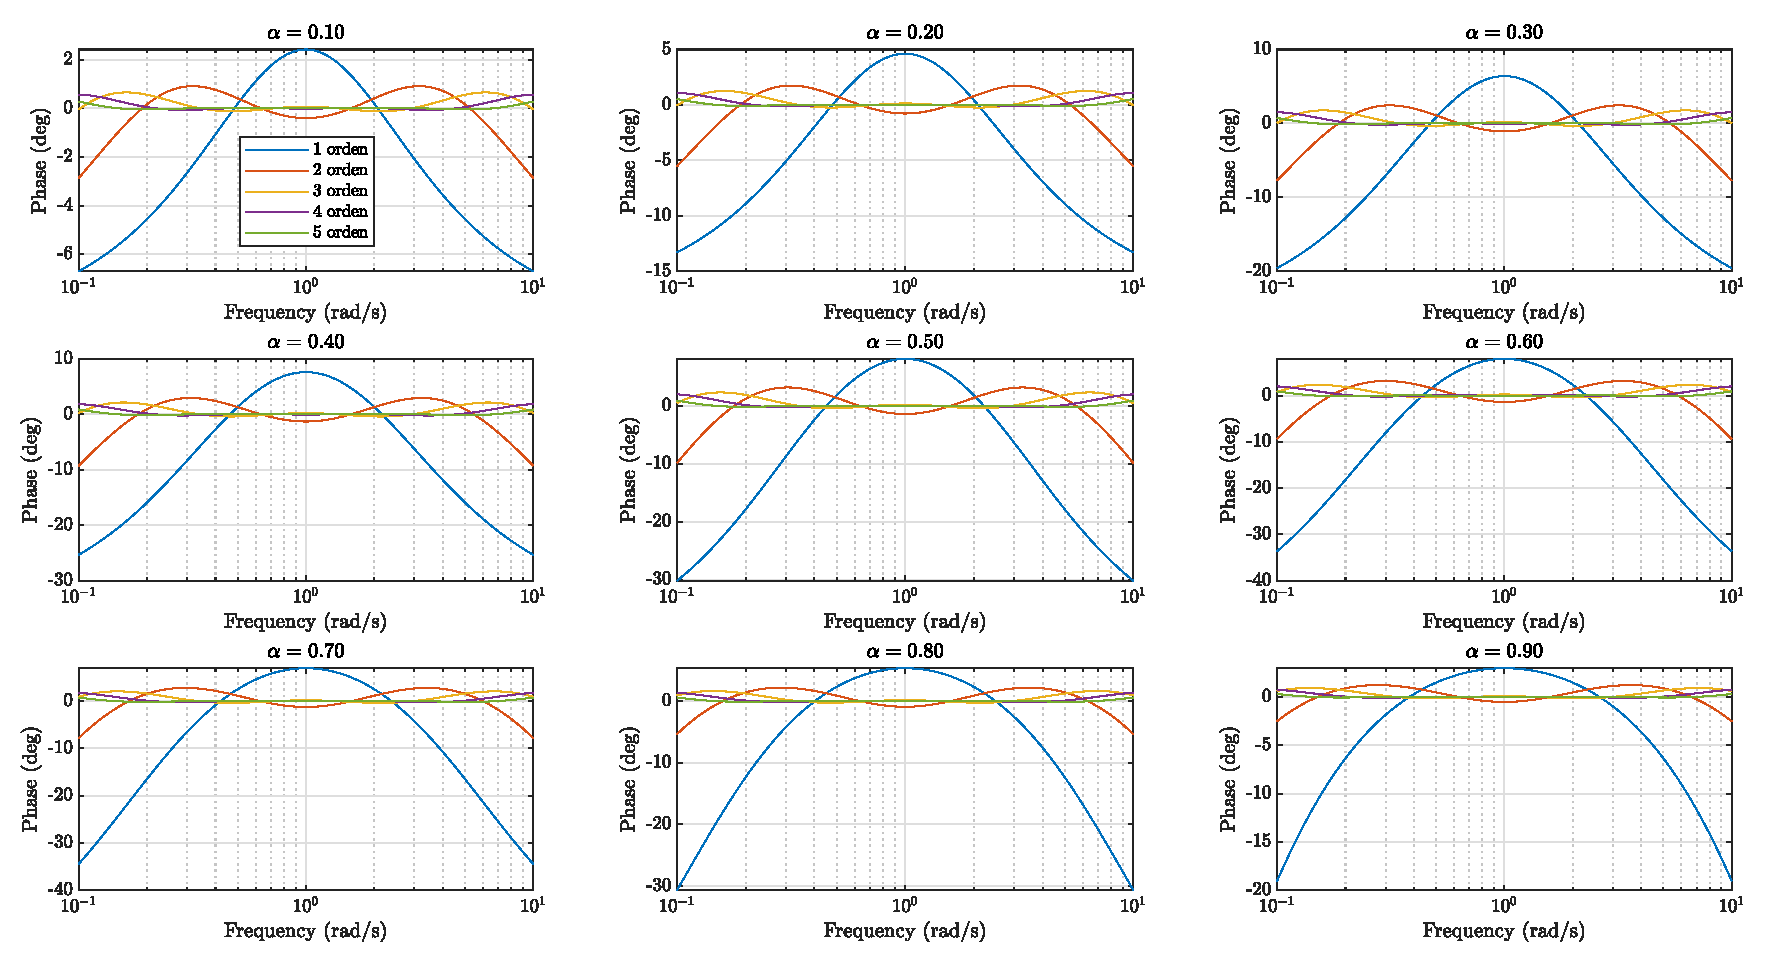
\includegraphics[width=0.93\textheight,angle=90]{F5_bode_error_fase_c.eps}
\end{figure}

%-------------------------------------------------------------------------------
%                            Graficas normalizadas                             %
%-------------------------------------------------------------------------------
\begin{figure}[hbtp]
	\caption{Diagramas de magnitud normalizada de aproximaciones de integrador fraccionario general.}
	\centering
	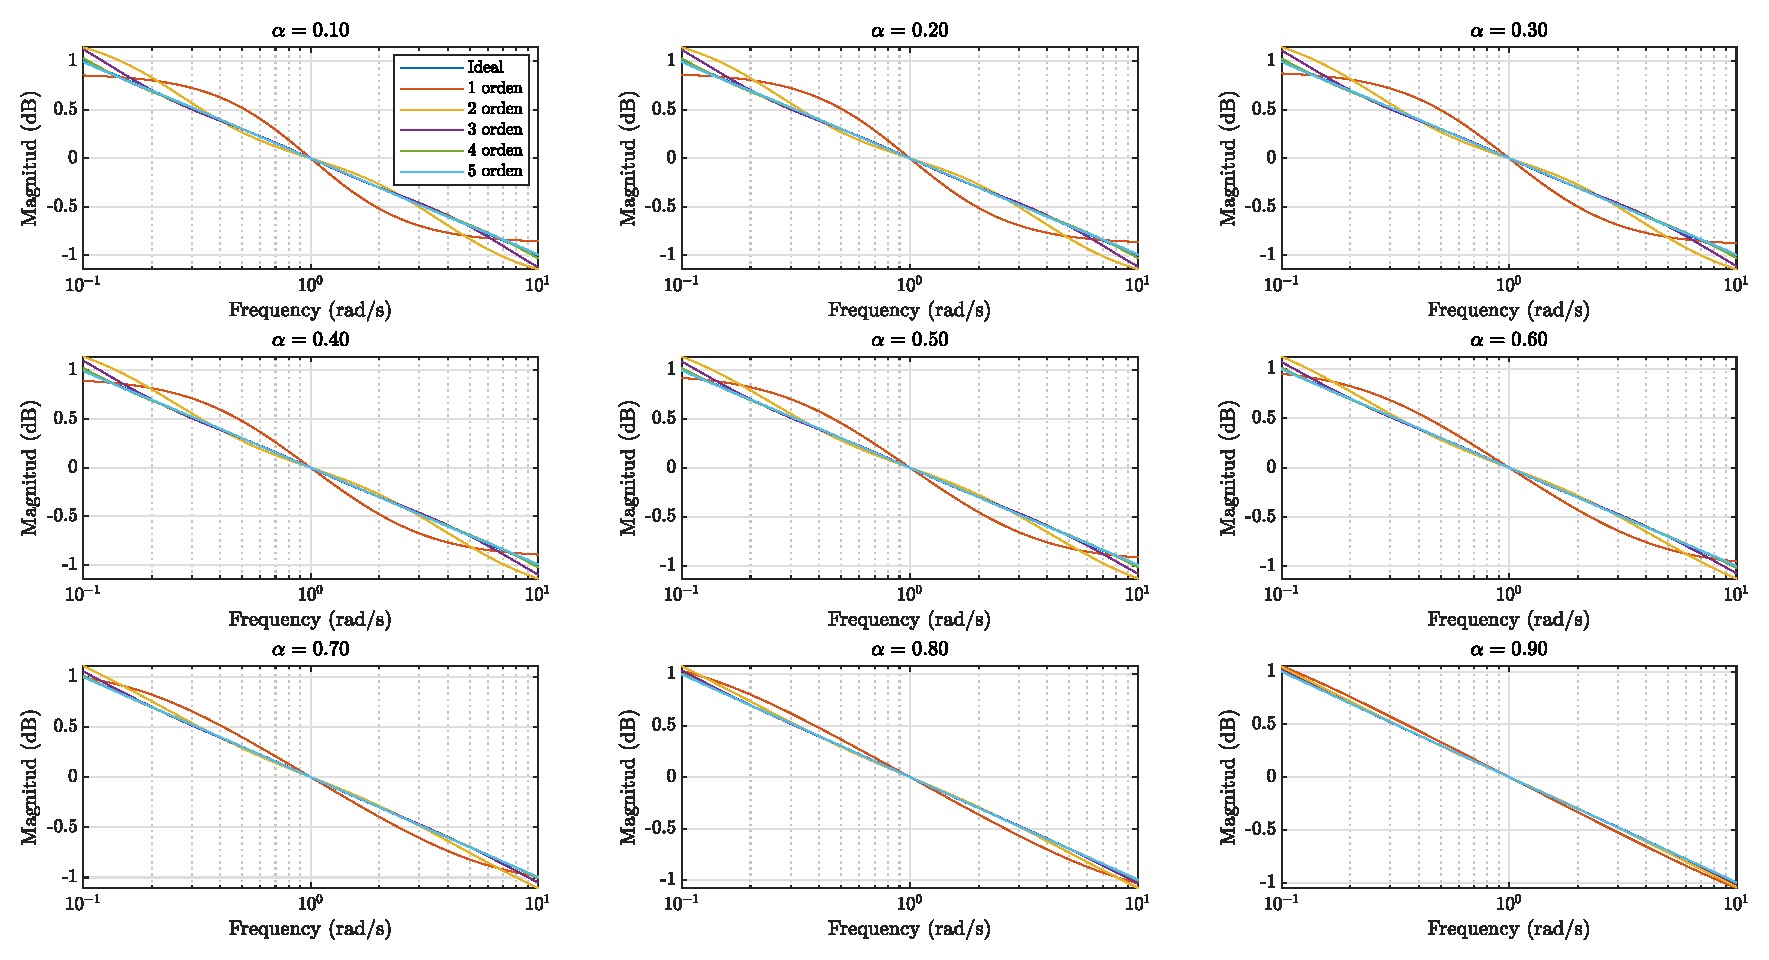
\includegraphics[width=0.93\textheight,angle=90]{F6_bode_magnitud_norm_c.eps}
\end{figure}

\begin{figure}[hbtp]
	\caption{Diagramas de fase normalizada de aproximaciones de integrador fraccionario general.}
	\centering
	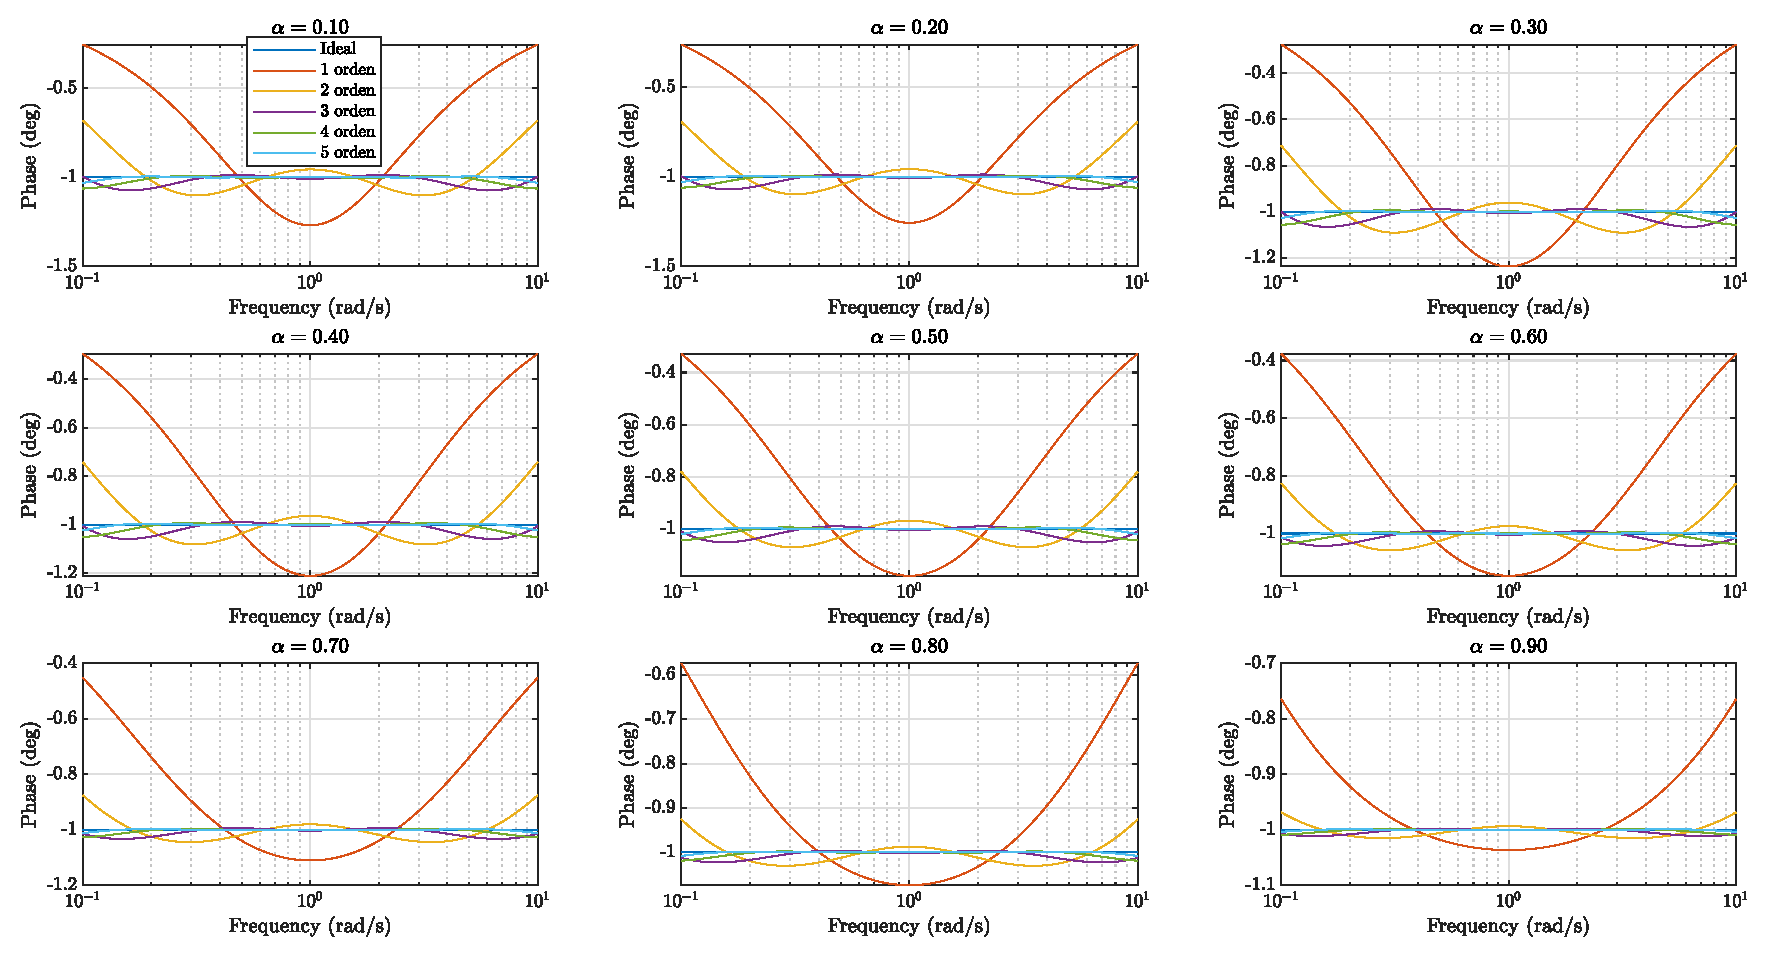
\includegraphics[width=0.93\textheight,angle=90]{F7_bode_fase_norm_c.eps}
\end{figure}

\begin{figure}[hbtp]
	\caption{Diagramas de error de magnitud normalizada de aproximaciones de integrador fraccionario general.}
	\centering
	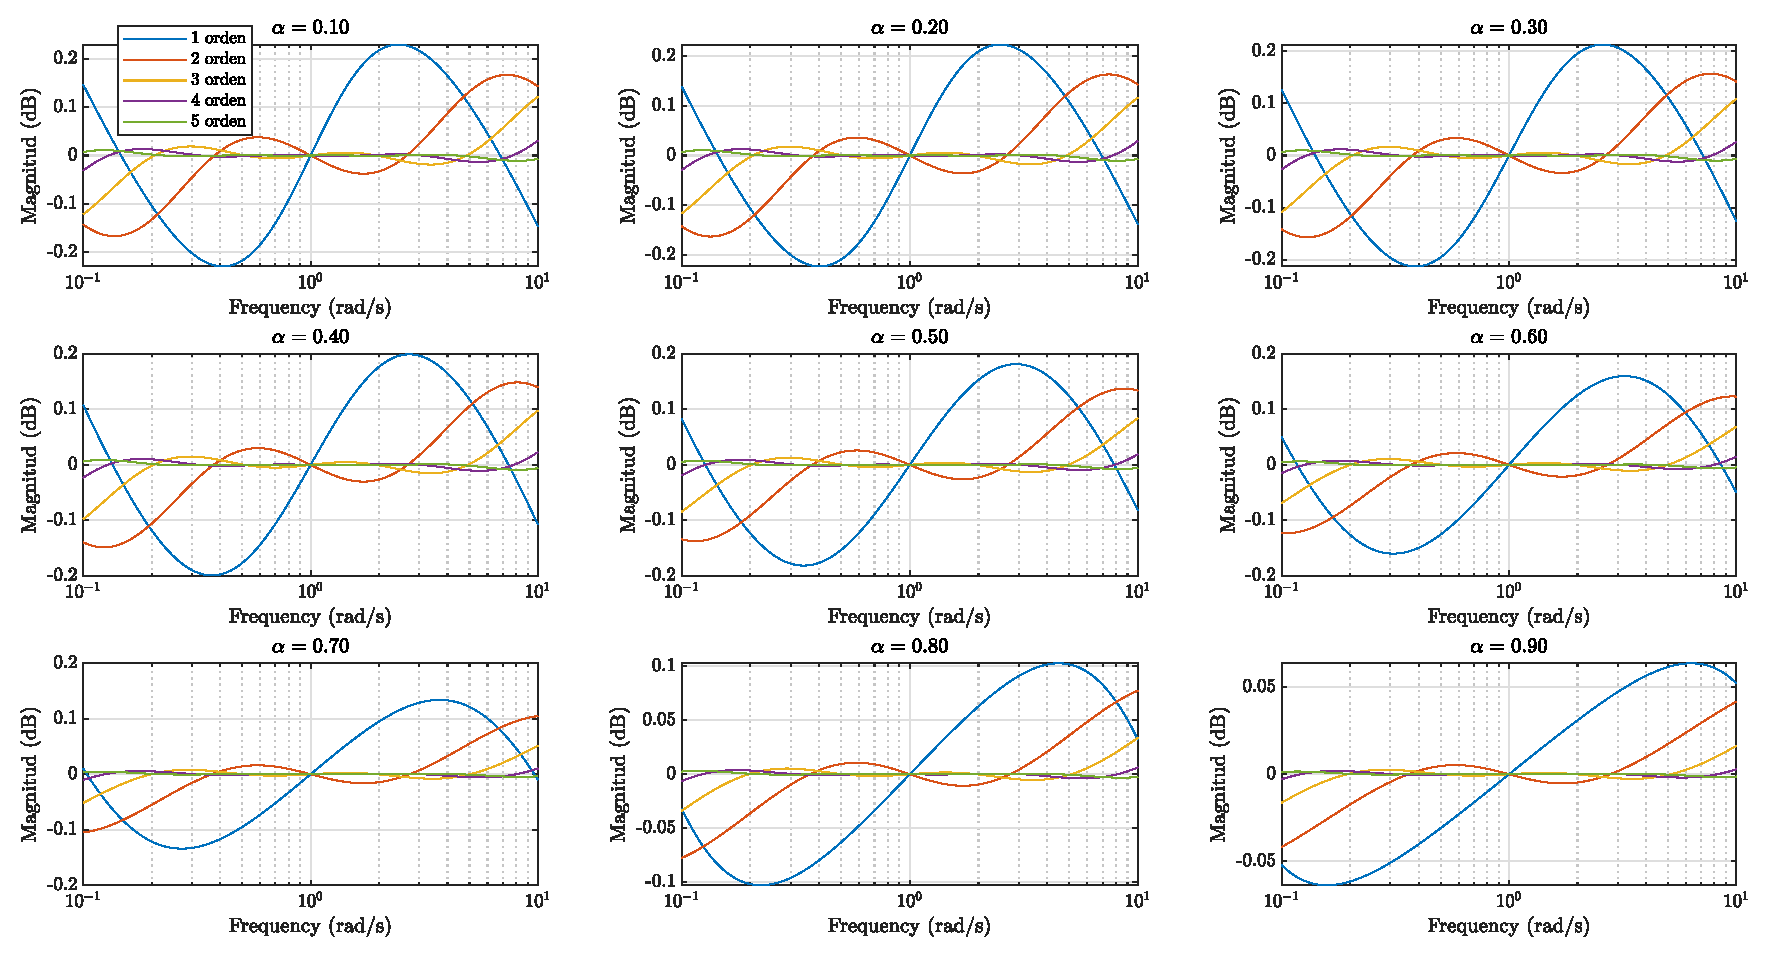
\includegraphics[width=0.93\textheight,angle=90]{F8_bode_error_mag_norm_c.eps}
\end{figure}

\begin{figure}[hbtp]
	\caption{Diagramas de error de fase normalizada de aproximaciones de integrador fraccionario general.}
	\centering
	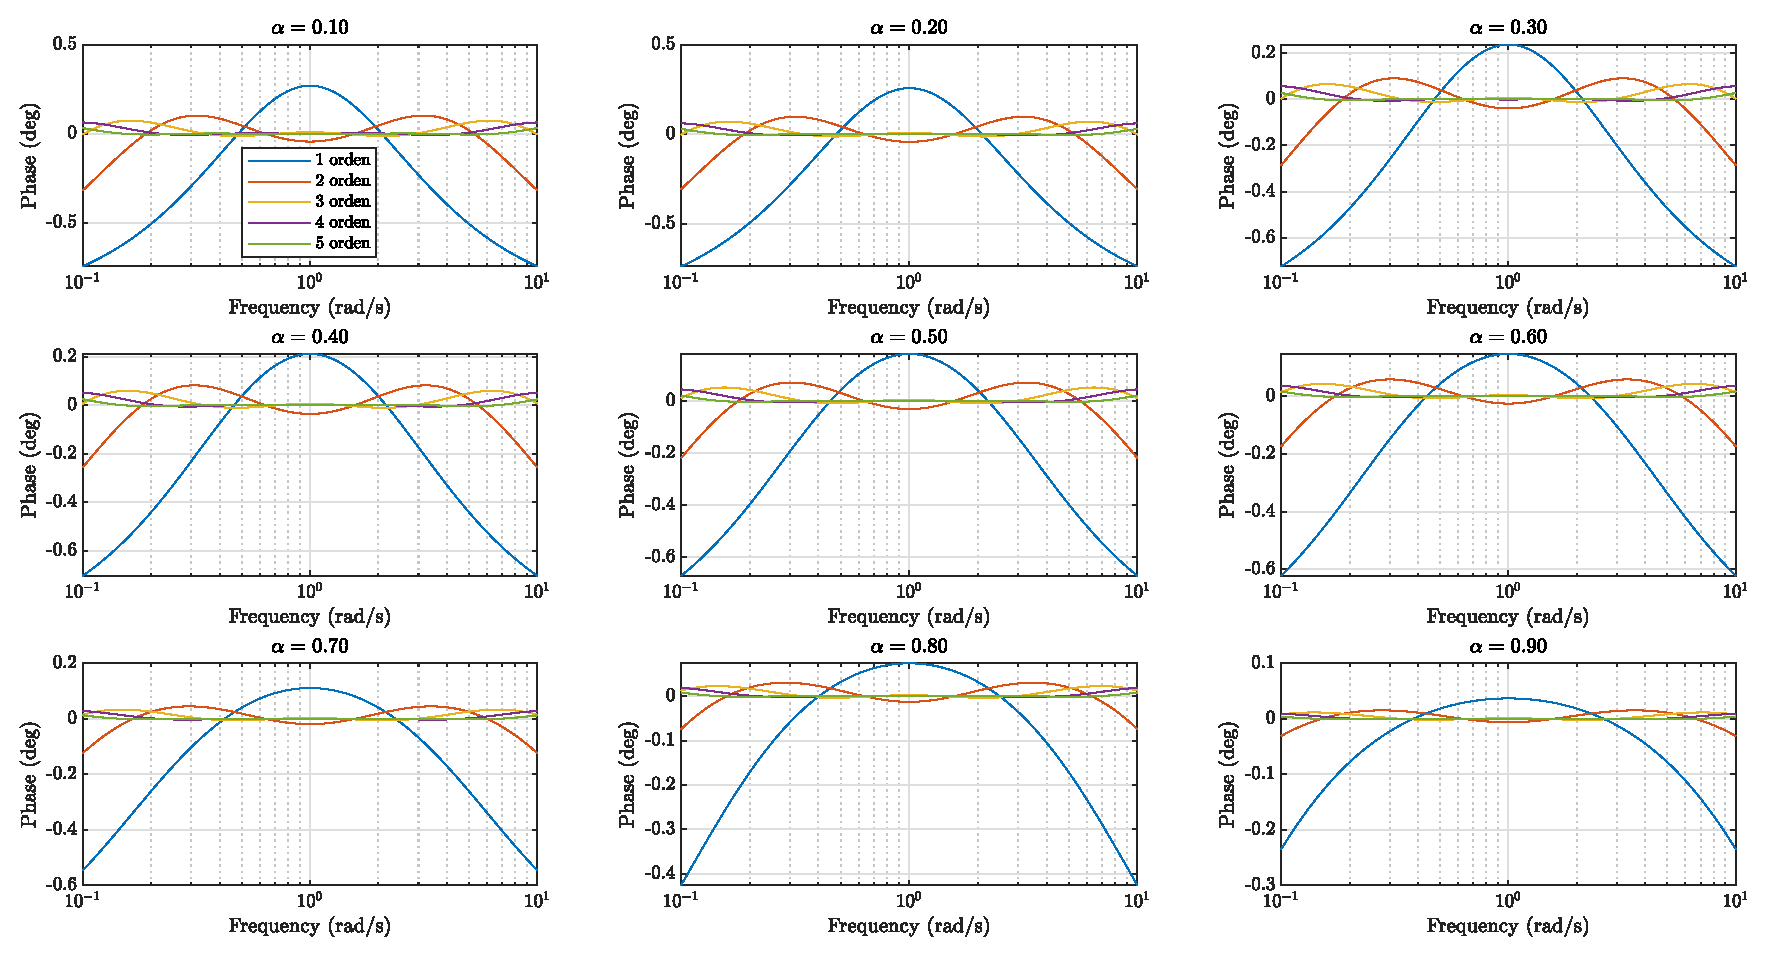
\includegraphics[width=0.93\textheight,angle=90]{F9_bode_error_fase_norm_c.eps}
\end{figure}